%# -*- coding: utf-8-unix -*-
%%==================================================
%% chapter01.tex for SJTU Master Thesis
%%==================================================

%\bibliographystyle{sjtu2}%[此处用于每章都生产参考文献]
\chapter{模拟研究}
\label{chap:analysis}

\section{案例背景}

随着我国经济的发展,我国市场与全球市场联系的越来越紧密,各类商品的市场化程度不断升高,我国实体企业在原材料或产成品的价格上的风险意识也逐渐增强,使用衍生产品对冲风险的需求与日俱增。期权作为一种衍生产品,在风险对冲上有着诸多的优势,可以满足企业对价格风险管理的需求。然而,我国场内期权市场刚刚起步,提供的场内期权产品从数量上或品种上难以满足这些企业的需求。因此,诸多期货公司和券商作为场外期权的交易商,通过场外市场为这些企业提供场外期权,帮助他们进行风险管理。

在场外期权市场中,交易商以提供流动性为主,通常处于净卖出期权的位置。并且,由于期权空头方的理论最大损失远大于期权多头方的理论最大损失,对于期权空头的对冲是交易商通常更为关心的。在之后的研究中,我们将以一家期货公司面临的模拟案例的形式,主要对期权空头方的动态对冲进行分析。

A公司是全国知名的发电集团,以火力发电为主,对动力煤有稳定的需求。某日,A公司下属某发电厂欲于60个交易日后购入动力煤100万吨。该公司管理层经过讨论认为,应使用衍生品工具对冲这批动力煤未来价格上涨的风险。然而,由于近期动力煤价格不稳定,未来价格存在着一定的下行空间。因此,公司不希望直接使用期货锁定动力煤价格,以至于会在动力煤价格发生大幅下跌时仍以之前锁定的、相对较高的价格购入。基于以上考量,A公司决定向B期货公司购入看涨期权进行对冲。假设动力煤现货价格为100元/吨,每手期权对应1吨动力煤,期权执行价100元,无风险利率为每年3\%,动力煤收益率的波动率为每年20\%,期权期限为60个交易日。使用BS模型,可以得出该期权价格约为每张4.24413元。B期货公司在出售这些看涨期权后,面临对冲问题。公司决定使用动态对冲的方法来对冲暴露的期权空头。

\section{研究方法}

根据上文的分析,动态对冲的具体执行逻辑如下:在初始时刻,根据期权头寸暴露的Delta,买卖相应数量的标的资产,并记录相应的现金成本。若为买入标的资产,则现金成本为正;若为卖出标的资产,现金成本为负。之后每个交易日,根据累计的现金成本,使用无风险利率计算当日的利息支出或收入,加总到现金成本中。之后进行再平衡条件的判断,若满足再平衡条件(达到了确定的再平衡时刻或组合的Delta的绝对值超过了设定的Delta阈值),则进行对组合的再平衡,将组合的Delta暴露调整为0,并类似地记录现金成本,直到到期日结束。到期日结束后,根据期权的行权情况,计算现金上的支出或收入,记入现金成本。最后,将总现金成本折现回初始日期,得到对冲成本。若有交易成本的话,只需在买卖标的资产时对应扣减相应的现金成本即可。

在对动态对冲结果的评价上,我们使用三个指标:期望对冲成本、相对对冲波动率和平均再平衡次数。对冲成本期望为模拟结果中对冲成本的平均值,对冲成本期望越小,说明场外期权空头方以此策略对冲的期望成本越小,策略越优。相对对冲波动为标准化后的对冲成本的标准差,具体计算方法为模拟结果中对冲成本的标准差除以期权的理论价格,相对对冲波动越小,说明场外期权空头方以此策略对冲的成本的波动越小,对于风险厌恶型的空头方来说策略越优。再平衡次数则会影响到交易成本的计算,同时也会带来隐性的操作成本。一般认为其他指标相同的情况下,再平衡次数越少,策略越优。同时,我们也会考察对冲成本的偏度,以对动态对冲策略的尾部风险有所认识。

基于以上期权的基本参数以及动态对冲的执行逻辑和结果评价指标,我们使用蒙特卡洛模拟的方法,进行了四十万次模拟。根据蒙特卡洛模拟的收敛速度,最终得到的一阶矩的误差应当在0.0005量级,本节之后所有的数值上的比较和结论均以此误差范围为前提。我们分别模拟了固定时点对冲策略和固定Delta区间对冲策略的对冲效果,将首先考察无交易费用时动态对冲的结果,以对动态对冲的结果有一个初步的、直观的认识,之后再加入不同的交易成本,对比得出交易成本对动态对冲的影响。最后,我们将基于模拟结果,讨论动态对冲策略和参数的选择问题,试图找出最优的对冲策略及其对应的参数。

\section{无交易费用时的动态对冲}

\subsection{固定时点动态对冲}

在固定时点动态对冲中,我们选取再平衡时间间隔分别为1天、3天、5天、10天和15天,对冲结果如下

\begin{table}[htbp]
  \centering
  \caption{无交易费用时固定时点动态对冲结果}
  \label{tab:fixed_time_0}
  \begin{tabular}{cccccc}
    \toprule
    再平衡时间间隔 & 1 & 3 & 5 & 10 & 15 \\
    \midrule
    期望对冲成本 & 4.24392 & 4.24806 & 4.25002 & 4.25724 & 4.25955 \\
    对冲成本标准差 & 0.42881 & 0.73248 & 0.93660 & 1.30162 & 1.57070 \\
    相对对冲波动率 & 0.10104 & 0.17259 & 0.22068 & 0.30669 & 0.37009 \\
    平均再平衡次数 & 59.00000 & 19.00000 & 11.00000 & 5.00000 & 3.00000 \\
    对冲成本偏度 & 0.20244 & 0.31600 & 0.39032 & 0.52075 & 0.60554 \\
    \bottomrule
  \end{tabular}
\end{table}

\begin{figure}[htb]
  \centering
  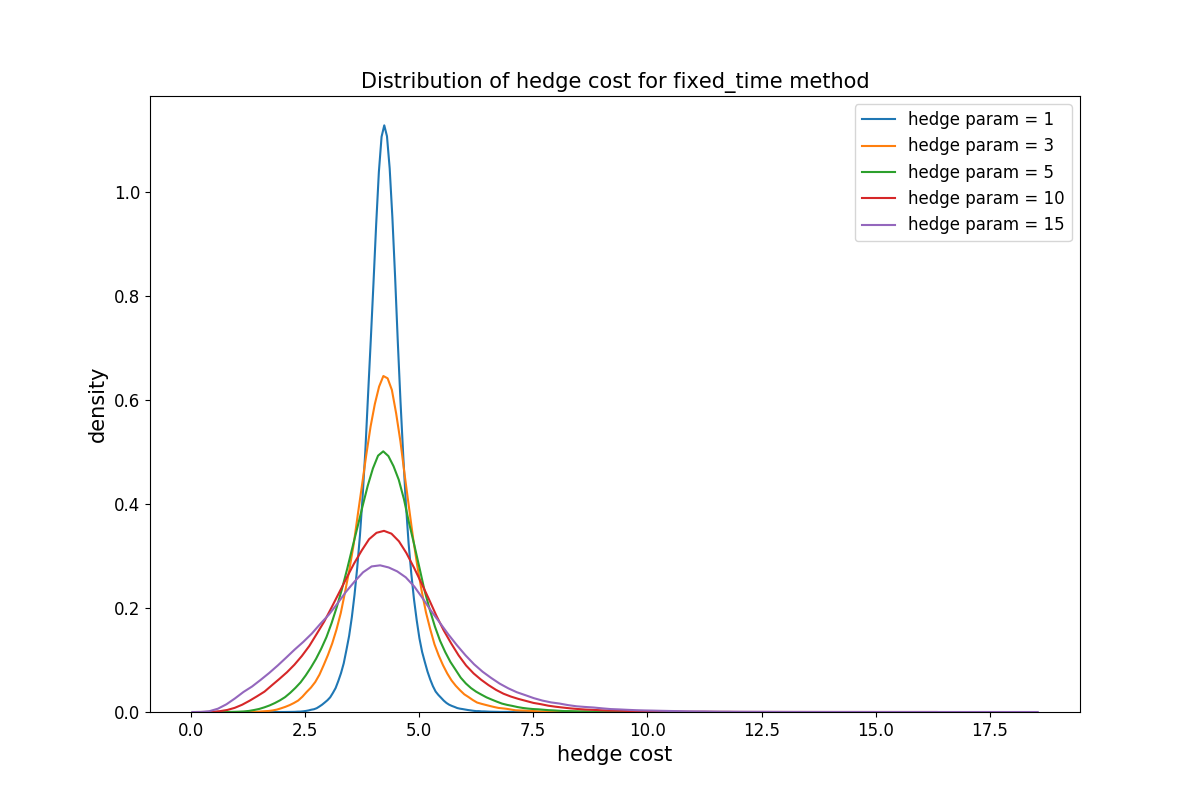
\includegraphics[width=12cm, height=8cm]{analysis/fixed_time_0_400000.png}
  \caption[这里将出现在插图索引中]
    {无交易费用时固定时点动态对冲对冲成本分布}
  \label{fig:fixed_time_0}
\end{figure}

从表\ref{tab:fixed_time_0}中,我们可以看出,随着再平衡频率的提高,对冲成本逐渐向BS模型计算出的理论价格收敛,并且相对对冲波动率逐渐减小,说明场外期权空头方的风险逐渐减小,最终的对冲成本变得更加"确定",对冲效果逐渐提高。这与BS模型的推导中的极限思想也是符合的。如果再平衡频率可以无限地提高,即再平衡时间间隔趋向于0,则期望对冲成本将依概率收敛到根据BS模型计算出的理论价格。虽然再平衡时间间隔为1天时的相对对冲波动率最低,对冲成本也最低,1天的再平衡时间间隔此时策略的最优参数,但是,其再平衡次数也达到了59次,若存在交易成本的话,频繁的再平衡将导致的交易成本的增加,这可能会提高对冲成本,使得其最终的期望对冲成本高于频率更低的情况。

图\ref{fig:fixed_time_0}展示了不同再平衡时间间隔下,对冲成本的分布情况。对冲成本的分布整体上呈现出右偏的特点。再平衡时间间隔越长时,对冲成本偏度越大,尾部风险较高,这可以从期权收益不对称的角度解释,同时也与动态对冲的具体的执行逻辑有关。Delta上的动态对冲在操作上其实是一个追涨杀跌的过程,最终的对冲成本取决于买入或卖出标的资产过程中标的资产的平均成交价格。随着到期日的临近,Gamma逐渐升高,由于再平衡时间较长,在两个再平衡时点之间如果标的价格出现了较强的单边趋势,则对冲组合的Delta相对于0的偏离值将会急剧增大,导致下一次再平衡时空头方需要以较高的价格买入大量标的资产对组合进行对冲。相比之下再平衡频率较高的情况,可以在标的出现单边趋势的过程中逐渐买入标的资产,最终标的资产的平均成交价格会相对较低,带来更低的对冲成本。因此,随着再平衡频率的提高,该动态对冲策略的尾部风险也会逐渐降低。

\subsection{固定Delta区间动态对冲}

在固定Delta区间动态对冲中,我们选取Delta阈值分别为0.03、0.05、0.1、0.15和0.2,对冲结果如下

\begin{table}[htbp]
  \centering
  \caption{无交易费用时固定Delta区间动态对冲结果}
  \label{tab:fixed_interval_0}
  \begin{tabular}{cccccc}
    \toprule
    Delta阈值 & 0.03 & 0.05 & 0.1 & 0.15 & 0.2 \\
    \midrule
    期望对冲成本 & 4.24618 & 4.24841 & 4.25352 & 4.26512 & 4.26066 \\
    对冲成本标准差 & 0.44593 & 0.48191 & 0.63572 & 0.83305 & 1.00841 \\
    相对对冲波动率 & 0.10507 & 0.11355 & 0.14979 & 0.19628 & 0.23760 \\
    平均再平衡次数 & 29.43722 & 20.25935 & 9.30494 & 5.20781 & 3.36678 \\
    对冲成本偏度 & 0.18198 & 0.14027 & 0.11910 & 0.22379 & 0.19918 \\
    \bottomrule
  \end{tabular}
\end{table}

\begin{figure}[htb]
  \centering
  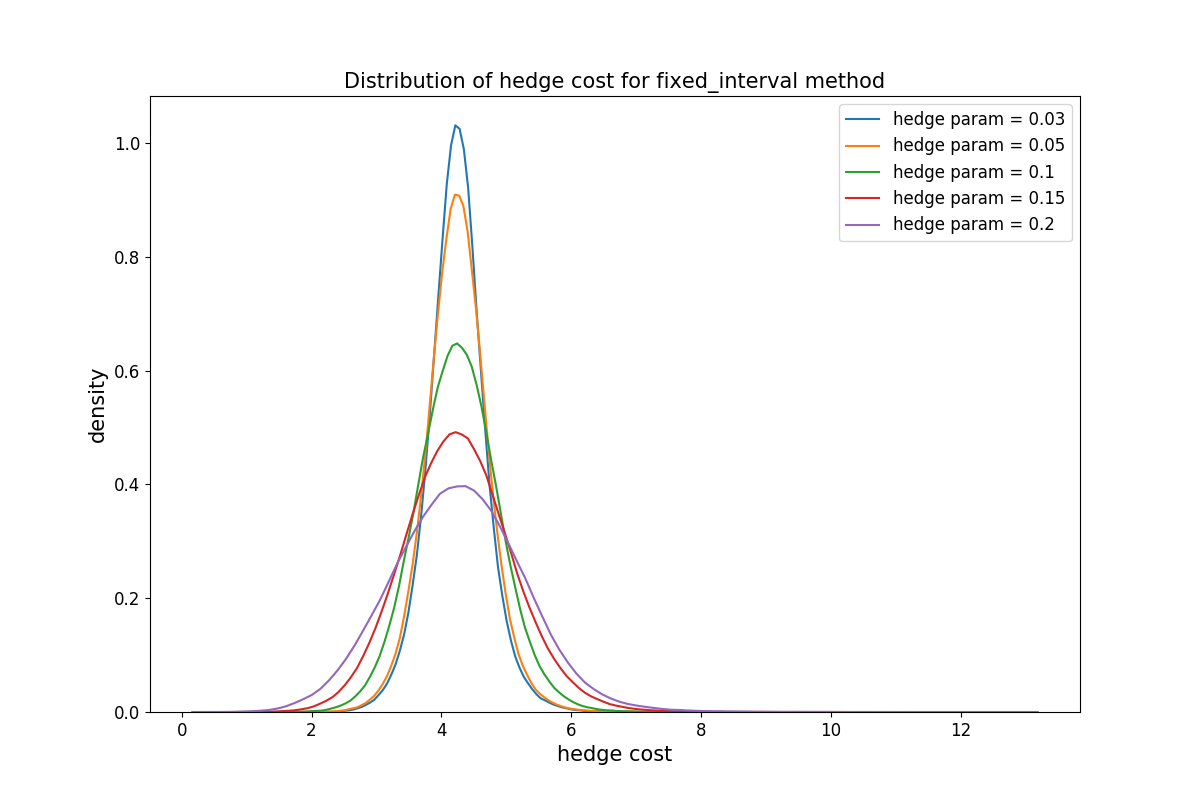
\includegraphics[width=12cm, height=8cm]{analysis/fixed_interval_0_400000.png}
  \caption[这里将出现在插图索引中]
    {无交易费用时固定Delta区间动态对冲对冲成本分布}
  \label{fig:fixed_interval_0}
\end{figure}

从表\ref{tab:fixed_interval_0}中,我们可以看出,随着Delta阈值的减小,对冲成本逐渐向BS模型计算出的理论价格收敛,并且相对对冲波动率逐渐减小,说明场外期权空头方的风险逐渐减小,最终的对冲成本变得更加"确定",对冲效果逐渐提高。类似的,Delta阈值为0.03时,对冲效果最好,但是此时的再平衡次数也最多。图\ref{tab:fixed_interval_0}中对冲成本的分布同样呈现出右偏的特点。但是,与固定时点对冲不同的是,随着Delta阈值的减小(对冲次数的增加),对冲成本偏度并没有出现递减的趋势。

\begin{table}[htbp]
  \centering
  \caption{无交易费用时固定Delta区间动态对冲结果}
  \label{tab:compare_two_0}
  \begin{tabular}{cccccc}
    \toprule
    Delta阈值/再平衡时间间隔 & 0.03/1 & 0.05/3 & 0.1/5 & 0.15/10 & 0.2/15 \\
    \midrule
    期望对冲成本百分比差异 & 0.05344\% & 0.00842\% & 0.08244\% & 0.18559\% & 0.02614\% \\
    相对对冲波动率绝对差异 & 0.40336\% & -5.90379\% & -7.08918\% & -11.04047\% & -13.24857\% \\
    \bottomrule
  \end{tabular}
\end{table}

将表\ref{tab:fixed_interval_0}和表\ref{tab:fixed_time_0}中平均再平衡次数最接近的结果进行对比,得到表\ref{tab:compare_two_0}。从该表中,我们发现在平均再平衡次数相差不大时(后四组结果),固定Delta区间对冲策略的期望对冲成本略高于固定时点对冲策略的期望对冲成本。这可以从两者在再平衡时需要对冲的Delta的值的分布得到解释。虽然两者对冲再平衡次数近似,但是对于固定Delta区间对冲来说,它每次再平衡时需要对冲的Delta一定会超过Delta阈值,因此其每次买入或卖出标的资产的量存在一个下界;而对于固定时点对冲,每次再平衡时需要对冲的Delta的绝对值不存在这样一个下界。因此在再平衡次数近似的情况下,前者的期望对冲成本会较高。同时,基于这一分析,固定Delta区间对冲对组合Delta的暴露控制的更好,因此其在相对对冲波动率的绝对数值上有很大提升。

再对比Delta阈值为0.03和再平衡时间间隔为1天的结果,两组结果的期望对冲成本和相对对冲波动率都差异不大,但是前者的平均再平衡次数在29次左右,而后者的再平衡次数达到了59次,这说明在有交易成本时,固定时点对冲的总对冲成本可能会高于固定Delta区间对冲。同时,固定Delta区间对冲策略的对冲成本偏度整体要小于固定时点对冲策略的对冲成本偏度。以上对比分析说明,在无交易成本时,固定Delta区间对冲策略的再平衡时点选择更为有效,其对冲效果要优于固定时点对冲策略,并且可以更好地减小尾部风险。

\section{有交易费用时的动态对冲}

在上一节,我们考察了无交易费用时,固定Delta区间对冲策略和固定时点对冲策略的对冲效果。在两个策略的分析中,我们都得出了再平衡次数越多,期望对冲成本越低,相对对冲波动率越低,对冲效果越好的结论。然而,在加入了交易费用后,再平衡次数越多,额外的交易成本也越多,因此对冲效果的比较结果可能会有所改变。本节我们将考察交易费用对对冲效果的影响。

我们采用固定比例的交易费用,分别选取0。02\%、0.05\%、0.08\%和0.1\%四个水平的交易成本,与上一节类似地进行动态对冲的模拟,模拟结果参见附录\ref{app:sim_fee_result}。我们将对表\ref{tab:fixed_time_0.02}到表\ref{tab:fixed_interval_0.1}的结果进行对比分析。

\subsection{交易费用对期望对冲成本的影响}

\begin{figure}[htb]
  \centering
  \subcaptionbox{固定时点动态对冲}[12cm]
    {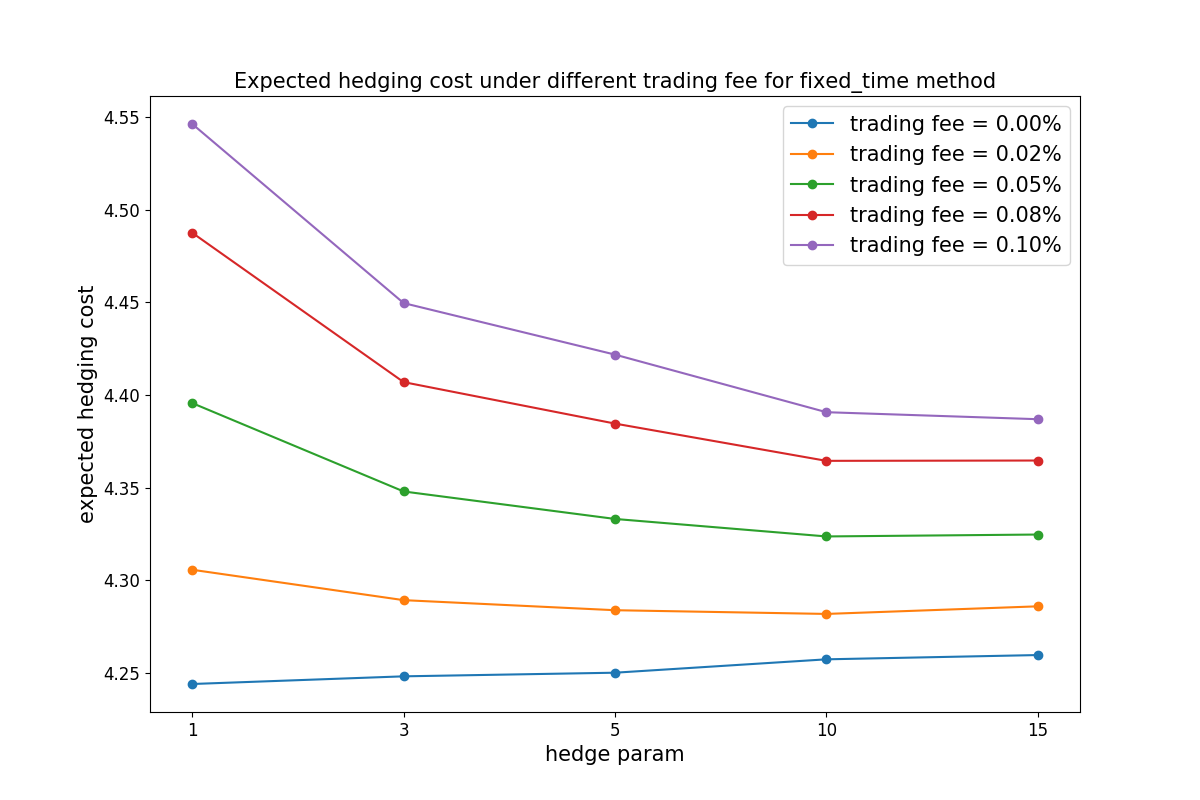
\includegraphics[width=12cm]{analysis/hedge_fee_fixed_time.png}}
  \hspace{0.5cm}
  \subcaptionbox{固定Delta区间动态对冲}[12cm]
    {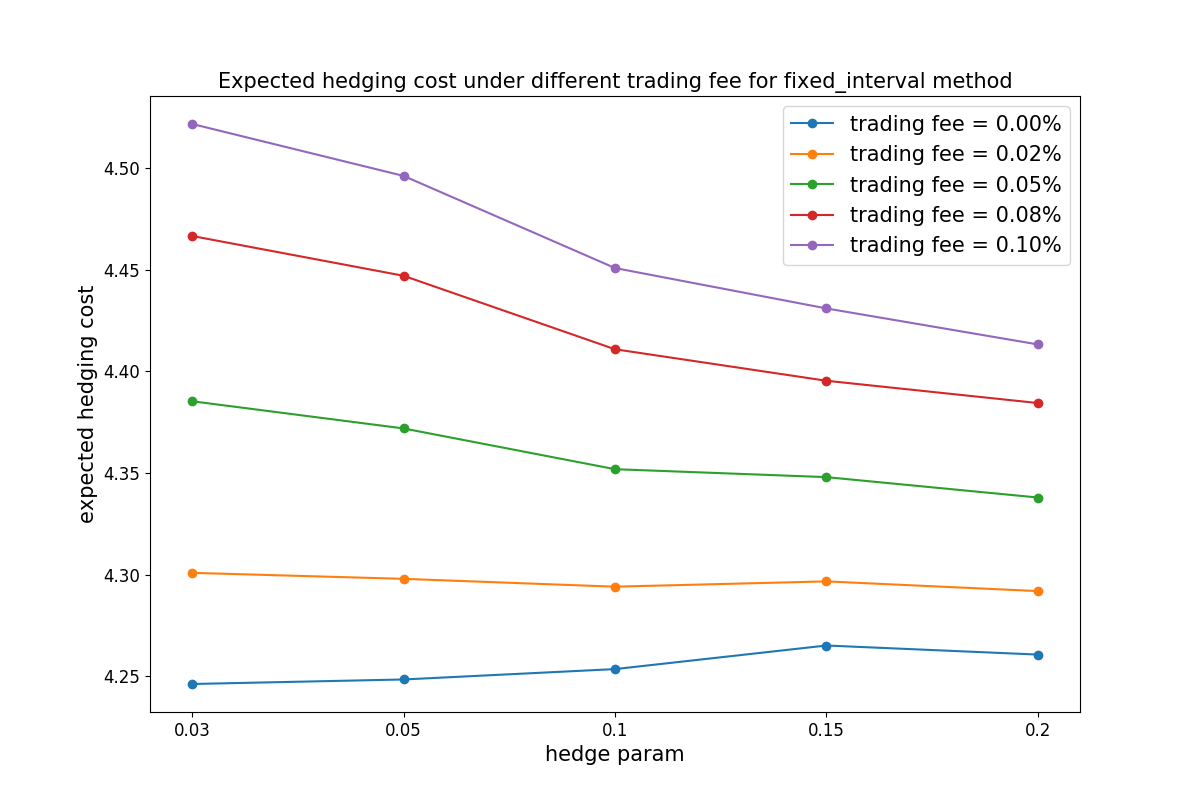
\includegraphics[width=12cm]{analysis/hedge_fee_fixed_interval.png}}
    \caption[这里将出现在插图索引中]
    {交易费用对期望对冲成本的影响}
  \label{fig:hedge_fee}
\end{figure}

图\ref{fig:hedge_fee}展示了不同交易费用对期望对冲成本的影响。引入交易费用将会增加期望对冲成本,其他条件相同的情况下,交易费用越高,期望对冲成本越高。

通过相同策略下每个表内结果的比较,我们发现随着平均再平衡次数的增加,期望对冲成本也基本上呈现出增加的趋势,但是并不严格单调。例如对于固定时点对冲策略,在交易费用较小时,存在一个再平衡时间间隔,其期望对冲成本为极值点,当再平衡时间间隔从该时间间隔增加或减小时,期望对冲成本总是增加。由于较长的再平衡时间间隔将带来较大的对冲误差,从而增加对冲成本,同时平均再平衡次数的增加也会增加交易费用从而对冲成本,因此在两者的共同作用下,将存在一个极值点,使其期望对冲成本最小。当交易费用较大时,其影响将占主要部分,此时期望对冲成本将会更严格地随平均再平衡次数递增。

通过不同策略,相同交易费用设定下结果的比较,我们发现平均再平衡次数相差不大的结果中(每张表的后四组结果),固定Delta区间对冲策略的期望对冲成本略高于固定时点对冲策略的期望对冲成本,幅度大概在0.5\%到1\%左右(相对于期权理论价格),这一期望对冲成本增加的原因在上一节有所提及。实际上,类似的平均再平衡次数下,固定Delta区间对冲策略中期望对冲成本的增加是对相对对冲波动率降低的一个“惩罚”,也正是由于该策略可以更有效地选择再平衡时刻,因此才会有更高的期望对冲成本和更低的相对对冲波动率。再比较每张表的第一组结果,我们发现在相对对冲波动率相差不大的情况下,固定Delta区间对冲策略下的期望对冲成本略低于固定时点对冲策略的期望对冲成本,这说明在该组结果的比较中,固定Delta区间对冲策略更优。

\subsection{交易费用对相对对冲波动率的影响}

\begin{figure}[htb]
  \centering
  \subcaptionbox{固定时点动态对冲}[12cm]
    {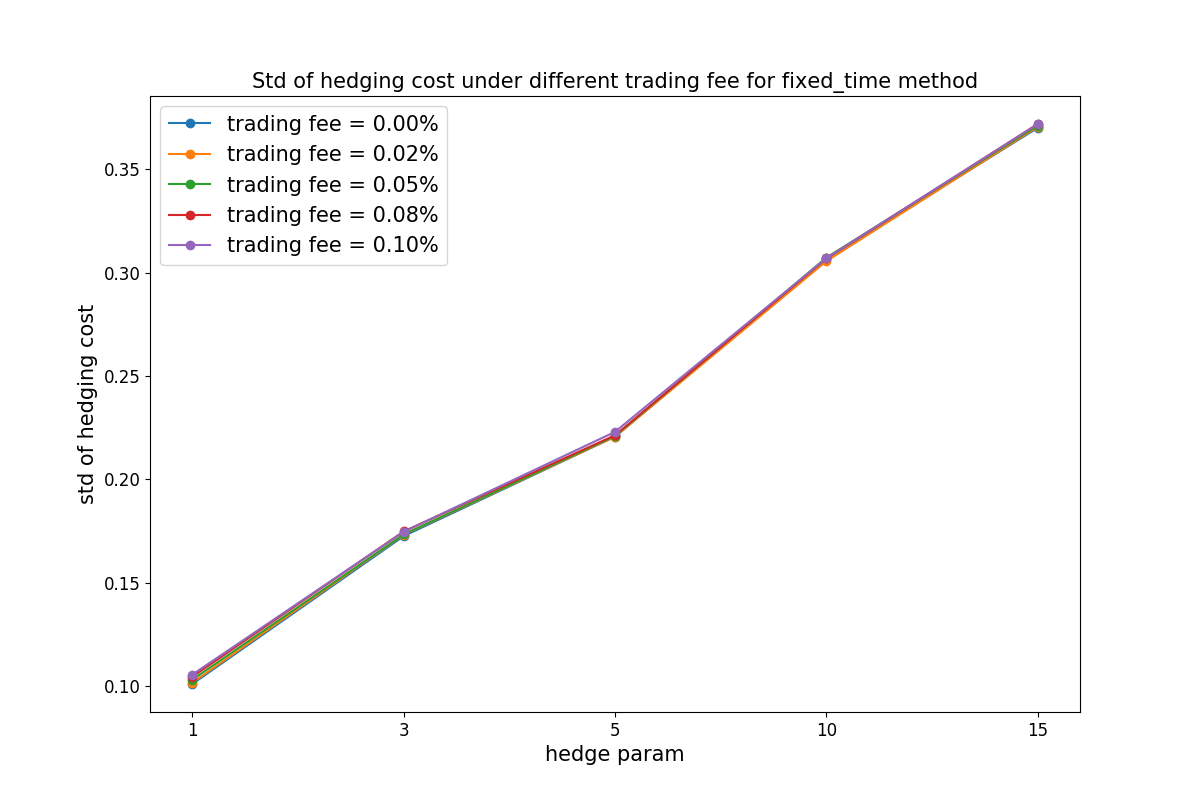
\includegraphics[width=12cm]{analysis/hedge_std_fixed_time.png}}
  \hspace{0.5cm}
  \subcaptionbox{固定Delta区间动态对冲}[12cm]
    {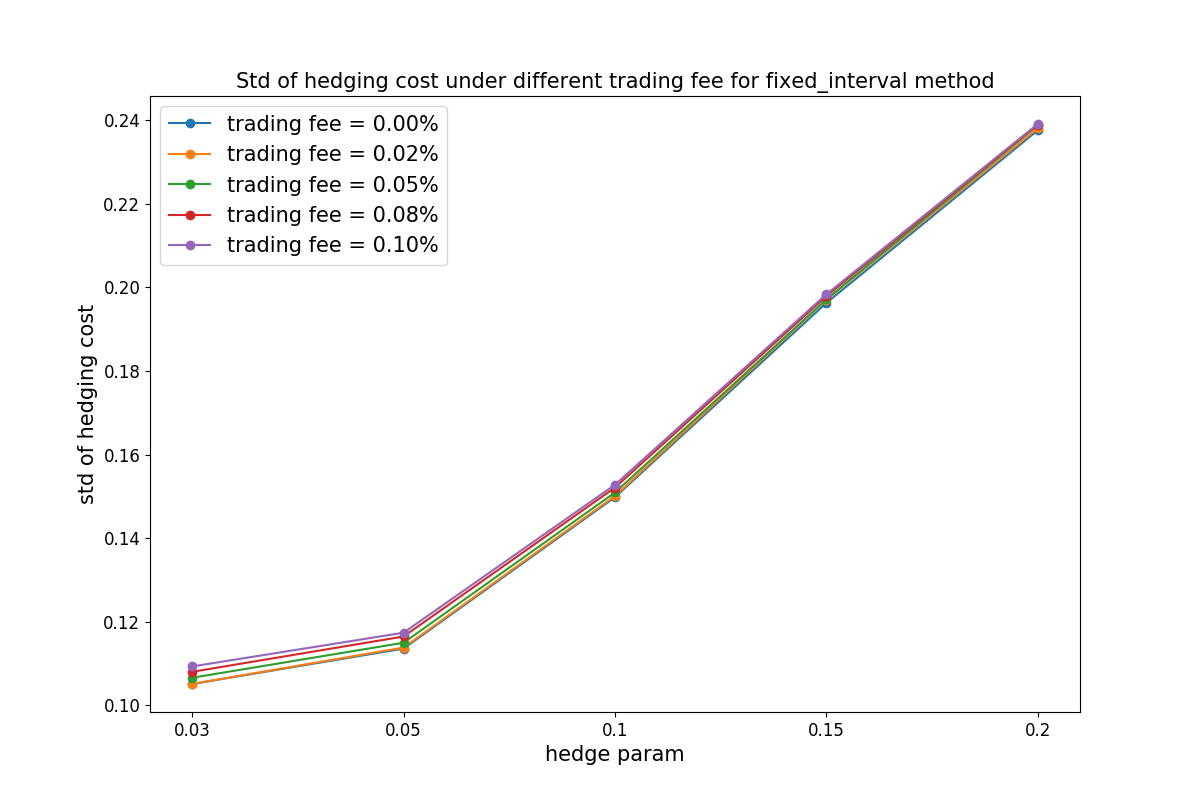
\includegraphics[width=12cm]{analysis/hedge_std_fixed_interval.png}}
    \caption[这里将出现在插图索引中]
    {交易费用对相对对冲波动率的影响}
  \label{fig:hedge_std}
\end{figure}

图\ref{fig:hedge_std}展示了不同交易费用对相对对冲波动率的影响。我们发现不同交易费用下,两个策略的相对对冲波动率水平和无交易费用时相差不大,但是基本呈现出随交易费用的增加而增加的趋势,这一现象在固定Delta对冲策略中Delta阈值为0.03时最为明显。由于我们使用的是成比例的交易费用,因此交易费用的引入相当于是成比例地增加了对冲成本,最终使得相对对冲波动率也会按照一定比例有所增加。

\subsection{交易费用对对冲成本偏度的影响}

\begin{figure}[htb]
  \centering
  \subcaptionbox{固定时点动态对冲}[12cm]
    {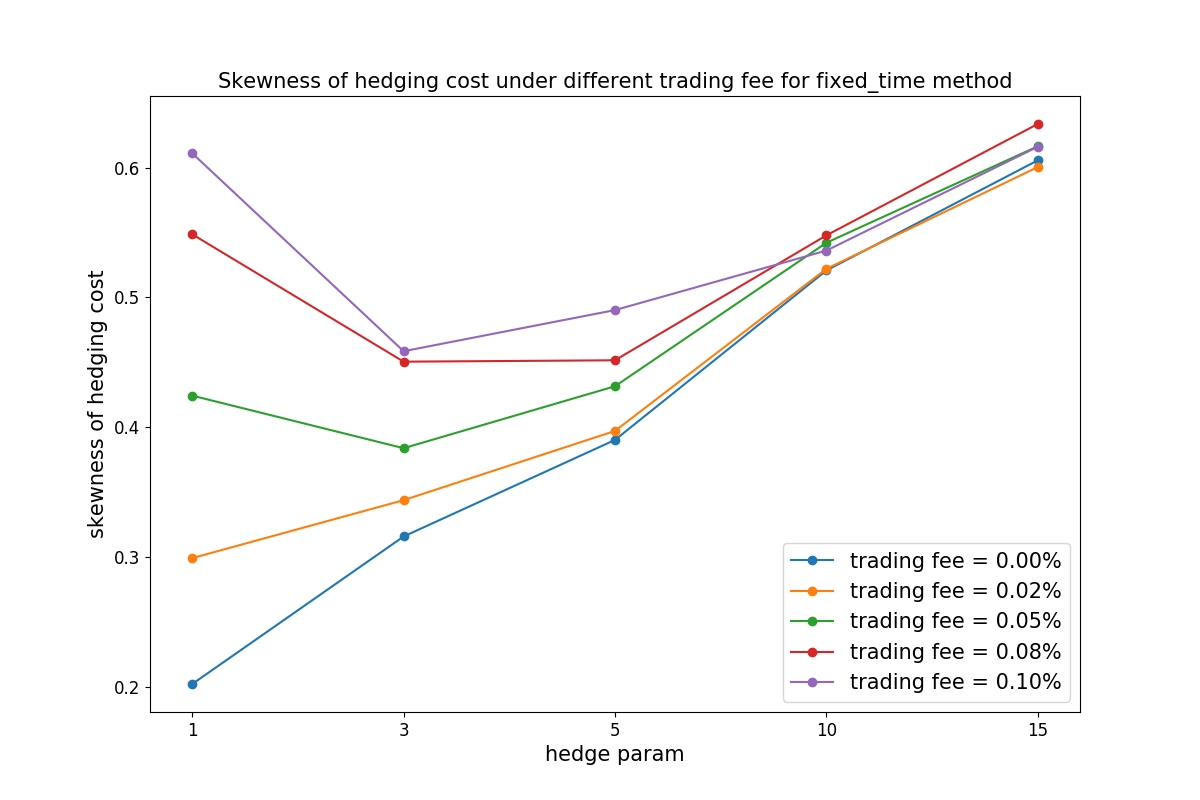
\includegraphics[width=12cm]{analysis/hedge_skew_fixed_time.png}}
  \hspace{0.5cm}
  \subcaptionbox{固定Delta区间动态对冲}[12cm]
    {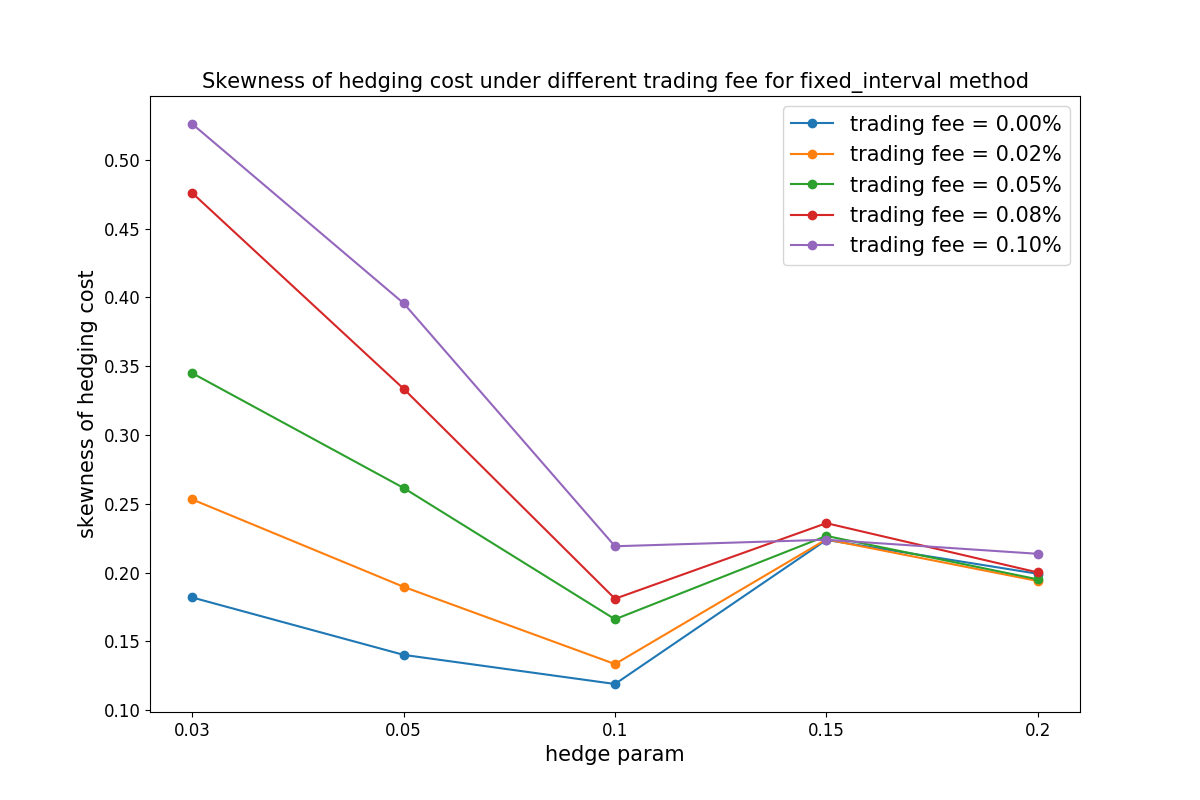
\includegraphics[width=12cm]{analysis/hedge_skew_fixed_interval.png}}
    \caption[这里将出现在插图索引中]
    {交易费用对对冲成本偏度的影响}
  \label{fig:hedge_skew}
\end{figure}

图\ref{fig:hedge_skew}展示了不同交易费用对对冲成本偏度的影响。我们发现交易费用的引入将显著地提升对冲成本的偏度。考察无交易费用时,处于右尾上的对冲成本对应的对冲操作。我们之前提到,这些对冲成本较高的情况一般是出现了较强的、不利的单边趋势。在这种情况下,场外期权空头方每次再平衡都需要买入(针对本章设定的卖出看涨期权情况)标的资产,交易费用的加入会带来更高的对冲成本;对于均值附近的对冲成本对应的动态对冲操作,这些情况下标的资产一般呈现震荡走势,空头方不需要在标的资产市场上进行数额较大的操作,额外的交易费用带来的对冲成本也会相对较小。因此,交易成本的引入将加剧原有对冲成本分布的右偏程度。并且,我们发现平均再平衡次数越高,对冲成本偏度的增加越明显,甚至会使得对冲成本偏度和平均再平衡次数的关系出现反转。这说明再平衡次数的增加带来的交易成本的增加对偏度影响要大于再平衡次数较少时对冲不精确的影响。

\section{动态对冲策略和参数选择}
\label{utility}

在上两节中,我们考察了有交易费用和无交易费用时,两个动态对冲策略的模拟结果。我们初步分析了对冲结果的期望对冲成本、相相对对冲波动率和对冲成本偏度,对不同参数下不同策略在这三个指标上的表现和变化特点有了初步的了解。本节我们将参考均值-方差效用函数,具体探讨如何根据以上指标,制定出动态对冲策略和参数选择的评判标准。

均值-方差效用函数的具体形式如下
\begin{equation}
  U=\mu+\frac{1}{2}\lambda\sigma^2
\end{equation}
其中,$\mu$为年化期望收益率,$\sigma$为年化收益率标准差,$\lambda$为风险偏好系数。当$\lambda$为负时,说明投资者是风险厌恶的,$\lambda$的绝对值越大,投资者的风险厌恶程度越高。本文假设场外期权交易商为风险厌恶者。

首先,我们定义对冲成本率为
\begin{equation}
  u=-(\frac{hc}{prc}-1)
\end{equation}
其中,$hc$为对冲成本,$prc$为期权的理论价格,$T_{total}$为期权的总期限。将其乘以一个年化系数即得到了年化对冲成本率。年化对冲成本率实际上代表了某种对冲策略下,相对于BS模型设定下的理想状态年化后的额外对冲成本。基于对冲成本率的概念,则$\mu$为年化期望对冲成本率,$\sigma$为年化对冲成本率标准差。利用之前提到的动态对冲的评价指标,我们可以得到适用于动态对冲策略分析的$\mu$和$\sigma$
\begin{equation}
  \mu=-(\frac{E[hc]}{prc}-1)\frac{252}{T_{total}}
  \label{eq:mu}
\end{equation}
\begin{equation}
  \sigma=rhv\sqrt{\frac{252}{T_{total}}}
  \label{eq:sigma}
\end{equation}
其中,$rhv$为相对对冲波动率,$E[hc]$为期望对冲成本。关于式\ref{eq:mu}和式\ref{eq:sigma}的具体推导见附录\ref{app:eq}。

我们以交易费用为万分之五为例,分析在这一对冲得分标准下,动态对冲策略和参数的选择。首先,固定时点对冲策略和固定Delta区间对冲策略的$\mu$和$\sigma$如下

\begin{table}[htbp]
  \centering
  \caption{动态对冲策略的$\mu$和$\sigma$}
  \label{tab:compare_two_0}
  \begin{tabular}{cccccc}
    \toprule
    Delta阈值/再平衡时间间隔 & 0.03/1 & 0.05/3 & 0.1/5 & 0.15/10 & 0.2/15 \\
    \midrule
    固定时点对冲策略的$\mu$ & -0.14990 & -0.10269 & -0.08800 & -0.07865 & -0.07967 \\
    固定Delta区间动态对冲策略的$\mu$ & -0.13965 & -0.12642 & -0.10659 & -0.10273 & -0.09281 \\
    固定时点对冲策略的$\sigma$ & 0.21130 & 0.35532 & 0.45301 & 0.62981 & 0.76059 \\
    固定Delta区间对冲策略的$\sigma$ & 0.21840 & 0.23557 & 0.30927 & 0.40400 & 0.48942 \\
    \bottomrule
  \end{tabular}
\end{table}

\begin{figure}[htb]
  \centering
  \subcaptionbox{固定时点动态对冲}[12cm]
    {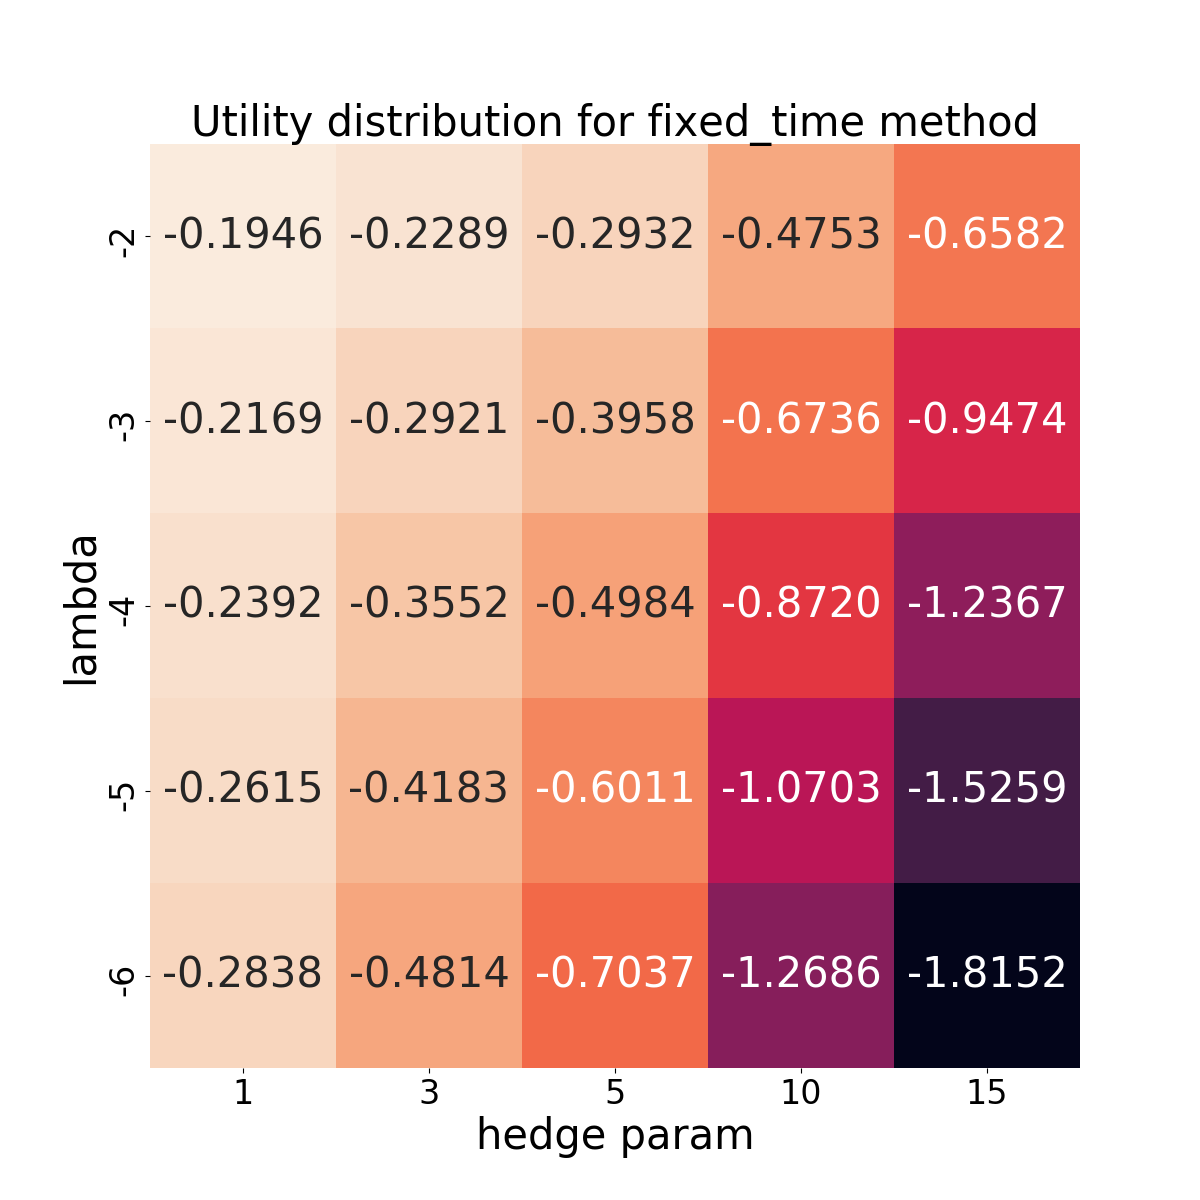
\includegraphics[width=7.5cm]{analysis/hedge_utility_fixed_time.png}}
  \hspace{0.5cm}
  \subcaptionbox{固定Delta区间动态对冲}[12cm]
    {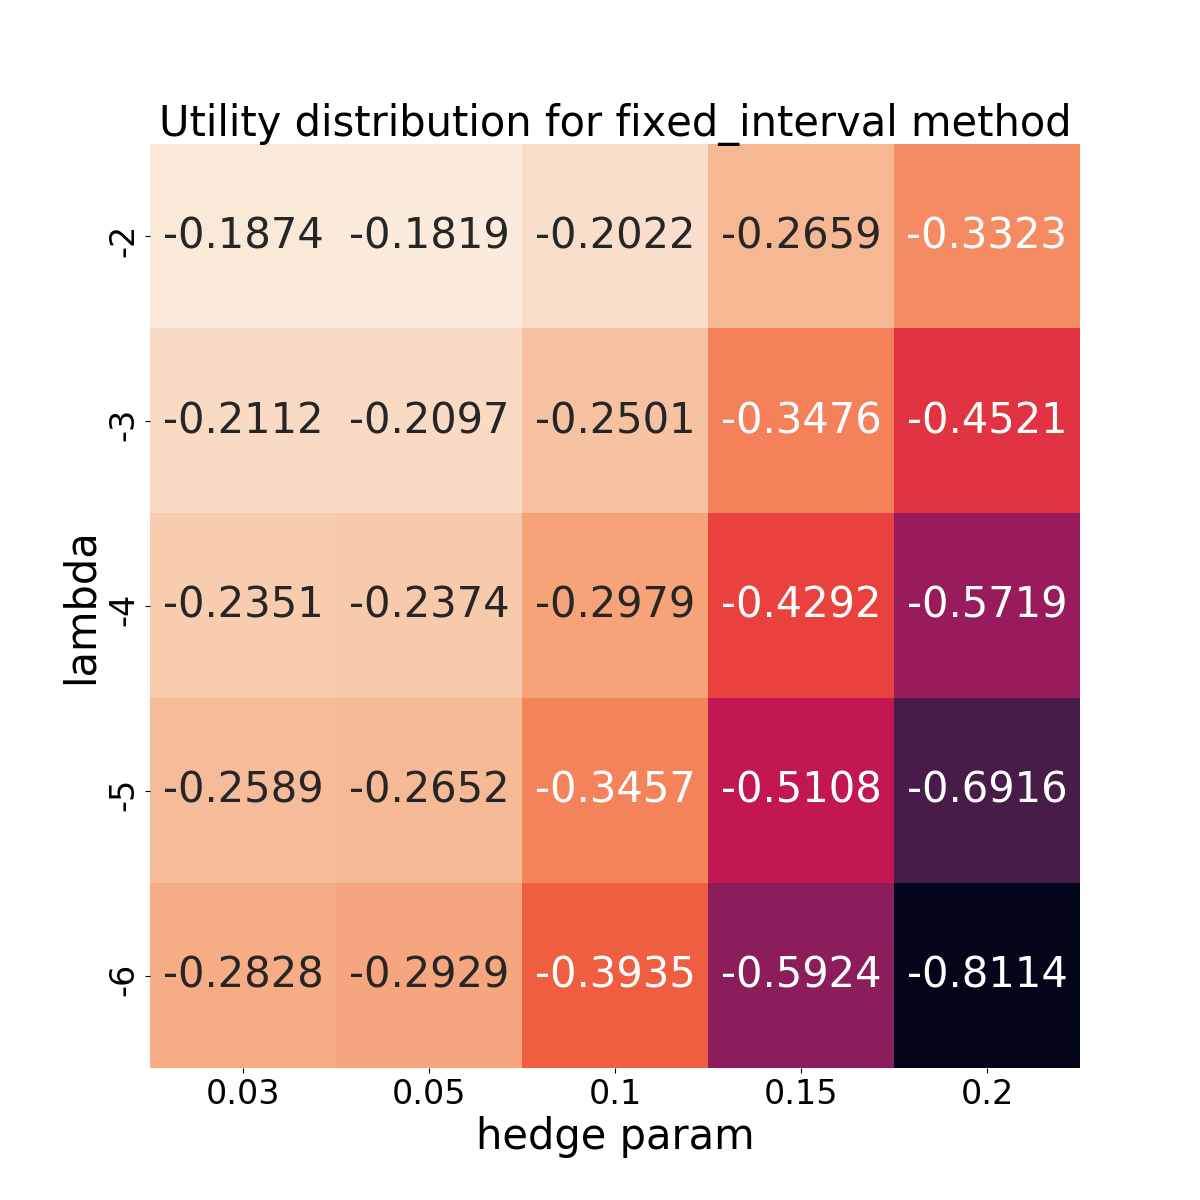
\includegraphics[width=7.5cm]{analysis/hedge_utility_fixed_interval.png}}
    \caption[这里将出现在插图索引中]
    {均值-方差对冲得分}
  \label{fig:hedge_utility}
\end{figure}

基于上述公式,我们设定$\lambda$为-2、-3、-4、-5和-6,计算得出两个策略的得分如图\ref{fig:hedge_utility}所示。从该图中可以看出,对于固定时点对冲策略,在固定$\lambda$值时,对冲得分总是和对冲参数呈负相关关系。这说明相比于对冲参数的改变带来的对冲成本的减少,这一评判标准认为其带来的在对冲成本波动率上的改进影响更大。因此,在给定的参数范围内,对于固定时点对冲策略,场外期权交易商应当选择再平衡时间间隔为1天。对于固定Delta区间对冲策略,结论大致与固定时点对冲相同。但是,我们发现在$\lambda$的绝对值小于或等于3时,Delta阈值为0.05的结果要优于Delta阈值为0。03的结果,当$\lambda$的绝对值大于3时,结果相反。这说明对于场外期权交易商而言,如果风险厌恶程度较低,则Delta阈值为0.05相对于0.03,在对冲成本上降低对最终对冲得分的影响效果要大于对冲成本波动率上的增加,交易商对期望对冲成本更为敏感;如果风险厌恶程度较高,则交易商会对对冲成本波动更为敏感,因此偏好Delta阈值为0.03的策略。但是总体上看,两个参数下策略表现相差不大。

横向对比固定时点对冲策略和固定Delta区间对冲策略,我们发现整体上来看固定Delta区间对冲策略的得分要高于固定时点对冲策略。这说明固定Delta区间对冲策略要优于固定时点对冲策略。并且,从两组策略对应位置的对冲得分差值随$\lambda$的变化中可以看出,场外期权交易商的风险厌恶程度越高,越偏好固定Delta区间对冲策略。

基于以上模拟研究,我们可以得出以下结论:场外期权交易商在对冲其看涨期权空头方向的暴露时,应当选择固定Delta区间对冲策略,具体阈值的选择取决于风险厌恶程度。

\section{本章小结}

本章以虚拟案例的形式,对动态对冲进行了模拟研究,主要考察动态对冲策略中各个参数以及交易成本对动态对冲结果的影响,同时对动态对冲的最优参数选择进行讨论。我们主要使用了期望对冲成本、相对对冲波动率和平均再平衡次数三个指标,也考察了对冲成本偏度。我们结合策略的操作特点对这些指标的表现进行了解释,并模仿均值-方差效用函数提出了一个动态对冲策略和参数选择的评判标准,同时基于这一标准对两个对冲策略在各个参数下的表现进行了评价,最终得出固定Delta区间对冲策略为更优的结论。在固定Delta区间策略中,具体阈值的选择取决于交易商的风险厌恶程度。
